\chapter{A Rule System for Analysis of Plan Change}
\label{cha:a-rule-system-for-analysis-of-plan-change}

A software product line may grow very large, and the plans even larger. Since different factors may influence the plan, it is necessary to be able to change the plan accordingly. If the plan is indeed extremely large, and since feature models have strict structure constraints, it is also necessary to have tool support that can check that the changes do not compromise the structure. Due to the size and complexity of the problem, it is not necessarily enough to let a human verify a change. 

To communicate our analysis method, we use rules similar to structural operational semantics rules.  The rules are on the form 
$$\sossize\begin{array}{c}
    \ntyperule{Rule-Label}
    { \\
    \text{Premises}}
    { S \transition S'}
  \end{array}$$
  where $S$ is the initial state, and $S'$ is the new state after the rule is applied. The rule can only be applied if all the premises hold. In the rules, the initial state is always on the form $\textbf{operation} \shove (\names{}, \features{}, \groups{})$, where \textbf{operation} denotes the change we intend to make to the interval-based feature model $(\names{}, \features{}, \groups{})$. The new state is always on the form $(\names{}', \features{}', \groups{}')$, where the maps have been updated according to the semantics of the operation. The premises ensure that an operation can only be applied if some conditions hold; for instance the $\rulefont{Add-Feature}$ rule \ref{rule:add-feature} contains premises verifying that the feature does not already exist when we wish to add it. The rules give us all the information we need to validate a modification, and to apply it.

\section{Add Feature Rule}
\label{sec:add-feature-rule}

\begin{figure}
    \renewcommand{\arraystretch}{1.1}
    \sossize$$\begin{array}{c}
      \ntyperule{Add-Feature}
      {\\
        \interval{t_n}{t_m} \not \innr F_e \qquad
        \interval{t_n}{t_m} \inn G_e \qquad
        \lookup{\lookup{\names{}}{\var{name}}}{\interval{t_n}{t_m}} = \emptyset \qquad
        t_n < t_m \\
        \lookup{\features{}}{\var{featureID}} = \feature \\
        \lookup{\groups{}}{\var{parentGroupID}} = \group\\
        \forall \var{gt} \in \lookup{G_t}{\interval{t_n}{t_m}} (\var{compatibleTypes}(\var{gt}, \var{type})) \\
      }
      {
        \textbf{addFeature}(\var{featureID}, \var{name}, \var{type}, \var{parentGroupID})\text{ from } t_n \text{ to } t_m\shove \\
         (\names{}, \features{}, \groups{})\\
        \transition\\
        (\lookup{\lookup{\names{}}{\var{name}}}{\interval{t_n}{t_m}} \assign \var{featureID},  \\
        \lookup{\features{}}{\var{featureID}} \assign 
        \var{setFeatureAttributes}(\lookup{\features{}}{\var{featureID}}, 
        \interval{t_n}{t_m}, \\
        \var{name}, \var{type}, \var{parentGroupID}),\\
        {\lookup{\groups{}}{\var{parentGroupID}}} \assign 
        \var{addChildFeature}(\lookup{\groups{}}{\var{parentGroupID}}, \interval{t_n}{t_m}, \var{featureID}))
    }
    \end{array}$$
    \caption{The \rulefont{Add-Feature} rule}
    \label{rule:add-feature}
\end{figure}

Recall from Section~\ref{sec:operations} that the \textbf{addFeature} operation adds a feature to the feature model evolution plan during a given interval. Figure \ref{rule:add-feature}  describes the semantics of the \textbf{addFeature} operation. 

When adding a feature during the interval $\interval{t_n}{t_m}$, its ID cannot be in use during the interval ($\interval{t_n}{t_m} \not \innr F_e$). The parent group must exist ($\interval{t_n}{t_m} \inn G_e$), and the types it has during the interval must be compatible with the type of the 
added feature ($\forall \var{gt} \in \lookup{G_t}{\interval{t_n}{t_m}} (\var{compatibleTypes}(\var{gt}, \var{type}))$). The name of the feature must not be in use during the interval ($\lookup{\lookup{\names{}}{\var{name}}}{\interval{t_n}{t_m}} = \emptyset$), and the interval must start before it ends ($t_n < t_m$). Notice that the default value in the $\features{}$ map lets us treat a failed lookup as a feature, thus allowing us to express the semantics of adding a feature using only one rule. When adding a feature, it may already exist in the plan during a different interval. In that case, we want to modify the existing feature entry. However, a feature being added is often completely new, and in that case it is useful that looking up the feature's ID in the \features{} map returns an empty feature entry $(\emptyset, \emptyset, \emptyset, \emptyset, \emptyset)$ instead of some undefined value, for instance $\bot$. This lets us treat both cases in the same way.

To make the rule tidier, we use three helper functions: $\var{compatibleTypes}$ (in Figure~\ref{fun:compatible-types}), $\var{setFeatureAttributes}$ (in Figure \ref{fun:set-feature-attributes}), and $\var{addChildFeature}$ (in Figure~\vref{fun:add-child-feature}). The $\var{compatibleTypes}$ function takes a group type (\andtype{}, \ortype{} or \xortype{}) and a feature type (\mandatory{} or \optional{}) and checks whether they are compatible. The types should belong to a parent group and its child feature. The only combination which is not allowed is a \mandatory{} feature with an \xortype{} or \ortype{} parent group.

The $\var{setFeatureAttributes}$ function takes a feature entry, an interval, a name, a type, and a group ID, and returns the feature entry with the information included. It modifies the existence set by adding the interval, maps the interval to the name in the names map, to the type in the types map, and to the parent group ID in the parent groups map.

The $\var{addChildFeature}$ function takes a group entry, an interval, and a feature ID, and adds the feature ID to the group's child feature map during the interval.

\begin{figure}[h]
  \begin{minted}[escapeinside=||]{text}
compatibleTypes(|$\andtype$|, _) = True
compatibleTypes(_, |$\optional$|) = False
compatibleTypes(_, _) = True
  \end{minted}
  \caption{\var{compatibleTypes}}
  \label{fun:compatible-types}
\end{figure}

\begin{figure}[h]
  \begin{minted}[escapeinside=||]{text}
setFeatureAttributes|$(\feature$|, |$\interval{t_{start}}{t_{end}}$|, name, type
                    , parentGroupID|$)$|
  = |$($| |$F_e \cup \set{\interval{t_{start}}{t_{end}}}$|
    , |$\lookup{F_n}{\interval{t_{start}}{t_{end}}}$| |$\assign$| name
    , |$\lookup{F_t}{\interval{t_{start}}{t_{end}}}$| |$\assign$| type
    , |$\lookup{F_p}{\interval{t_{start}}{t_{end}}}$| |$\assign$| parentGroupID
    , |$F_c \ )$|
   \end{minted}
  \caption{\var{setFeatureAttributes}}
  \label{fun:set-feature-attributes}
\end{figure}

\begin{figure}[h]
  \begin{minted}[escapeinside=||]{text}
addChildFeature|$(\group, \interval{t_{start}}{t_{end}}, \var{fid})$|
  = |$\left(G_e, G_t, G_p , \lookup{G_c}{\interval{t_{start}}{t_{end}}} \addassign \var{fid}\right)$|
  \end{minted}
  \caption{\var{addChildFeature}}
  \label{fun:add-child-feature}
\end{figure}

\subsubsection{Applying the \rulefont{Add-Feature} rule to an example}

We show how to use a rule by applying the \rulefont{Add-Feature} rule to a simple example. Following is a simple interval-based feature model, containing one feature and one group. The module is visualised in a simplified version in Figure~\vref{ex:add-feature-original-plan}. The visualisation shows only the structure of the feature model, not the feature or groups' types or other attributes.

\begin{align*}
  (&\; \{  \mapping{\text{Root}}{\set{\intervalmapping{1}{\forever}{\text{feature:root}}}} \\
   &\; \}\\
    ,&\; \{  \text{feature:root} \mapsto \left( \begin{aligned}
          \, & \set{\interval{1}{\forever}} \\
       ,  \, & \set{\intervalmapping{1}{\forever}{\text{Root}}} \\
       ,  \, & \set{\intervalmapping{1}{\forever}{\mandatory}} \\
       ,  \, & \emptyset \\
       ,  \, & \set{\intervalmapping{1}{\forever}{\set{\text{group:A}}}} \\
  \end{aligned}\right) \\
   &\; \}\\ 
          ,&\; \{ \text{group:A} \mapsto \left( \begin{aligned}
                & \set{\interval{1}{5}} \\
                , \, & \set{\intervalmapping{1}{5}{\andtype}} \\
                , \, & \set{\intervalmapping{1}{5}{\text{feature:Root}}} \\
                , \, & \emptyset \\
            \end{aligned} \right) \\
   &\; \})
\end{align*}

\begin{figure}[h]
  \centering
  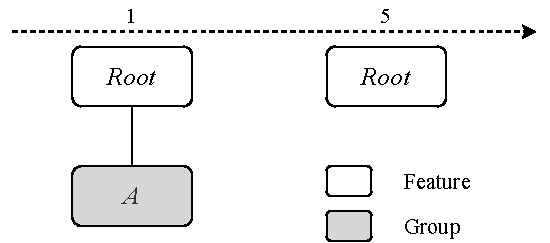
\includegraphics[width=0.7\textwidth]{AddFeatureOriginalPlan}
  \caption{Add feature example \textemdash{} original plan}
  \label{ex:add-feature-original-plan}
\end{figure}

We apply the operation \textbf{addFeature}$(\text{feature:B}, \text{B}, \optional{}, \text{group:A})$ from $3$ to $5$ using the \rulefont{Add-Feature} rule. This means that we want to add a feature with ID feature:B, name B, and type \optional{} to the group with ID group:A from time 3 until (but not including) 5. We must go through all the premises and check that each of them holds for the original model. First, we look up the new feature in the original model. Since the feature does not exist, we get
\[
  \lookup{\features{}}{\text{feature:B}} = (\emptyset, \emptyset, \emptyset, \emptyset, \emptyset)
\]
We further look up the parent group:
\begin{align*}
  \lookup{\groups{}}{\text{group:A}} = ( 
                & \set{\interval{1}{5}} \\
                , \, & \set{\intervalmapping{1}{5}{\andtype}} \\
                , \, & \set{\intervalmapping{1}{5}{\text{feature:Root}}} \\
                , \, & \emptyset ) \\
\end{align*}
We see that the group exists from 1 to 5, that it has the type \andtype{} during its lifespan, and that its parent feature has ID \text{feature:Root}. Now that we have the information we require, we can check that the other premises hold.

In the premise $\interval{t_n}{t_m} \not \innr F_e$, we replace $t_n$, $t_m$ and $F_e$ by their concrete values:
\[
  \interval{3}{5} \not \innr \emptyset
\]
Since no element is member of $\emptyset$, no element in $\emptyset$ overlaps $\interval{3}{5}$, so this premise holds.

The premise $\interval{t_n}{t_m} \inn G_e$ asserts that an interval in $G_e$ should contain the interval $\interval{t_n}{t_m}$. We instantiate the variables with our concrete values and verify that this holds:
\[
  \interval{3}{5} \inn \set{\interval{1}{5}}
\]
Since $\interval{1}{5}$ does contain $\interval{3}{5}$, this premise also holds.

The premise $\lookup{\lookup{\names{}}{\var{name}}}{\interval{t_n}{t_m}} = \emptyset$ means that the name of the new feature should be unique during the temporal scope.  We verify:
\[
  \lookup{\lookup{\names}{\text{B}}}{\interval{3}{5}} = \emptyset
\]

The only key in the $\names{}$ map is A, so this statement is true. The next premise we check is $t_n < t_m$, which is true because $3 < 5$.

Lastly, we check that the types of the new feature and its parent group are compatible, the premise $\forall \var{gt} \in \lookup{G_t}{\interval{t_n}{t_m}} (\var{compatibleTypes}(\var{gt}, \var{type}))$. We instantiate the variables:
\[
  \forall \var{gt} \in \lookup{\set{\intervalmapping{1}{5}{\andtype}}}{\interval{3}{5}}(\var{compatibleTypes}(\var{gt}, \optional{}))
\]
The only value in $\set{\intervalmapping{1}{5}{\andtype}}$ during the interval $\interval{3}{5}$ is \andtype, so we instatiate $\var{gt}$ with that value.
\[
  \var{compatibleTypes}(\andtype{}, \optional{})
\]
This matches the first case in the \var{compatibleTypes} function, which evaluates to \texttt{True}. Thus the last premise holds, so we can apply the transition. We go through each map individually, starting with \names{}. The rule gives the modification
\[
  \lookup{\lookup{\names{}}{\var{name}}}{\interval{t_n}{t_m}} \assign \var{featureID}
\]
which becomes
\[
  \lookup{\lookup{\{  \mapping{\text{Root}}{\set{\intervalmapping{1}{\forever}{\text{feature:root}}}}\}}{\text{B}}}{\interval{3}{5}} \assign \text{feature:B}
\]
This gives us the map
\begin{align*}
  \{\mapping{\text{Root}}{& \set{\intervalmapping{1}{\forever}{\text{feature:root}}}}, \\
   \mapping{\text{B}}{& \set{\intervalmapping{3}{5}{\text{feature:B}}}}\} 
\end{align*}
According to the rule, the \features{} map should be modified in the following way:
\begin{align*}
  \lookup{\features{}}{\var{featureID}} \assign \var{setFeature}&\var{Attributes}(\lookup{\features{}}{\var{featureID}}, \\
                           &\interval{t_n}{t_m},\\
                           &\var{name}, \var{type}, \var{parentGroupID})
\end{align*}
We instantiate:
\begin{align*}
  \lookup{\features{}}{\text{feature:B}} \assign \var{setFeature}&\var{Attributes}((\emptyset, \emptyset, \emptyset, \emptyset, \emptyset), \\
                           &\interval{3}{5},\\
                           &\text{A}, \optional{}, \text{group:A})
\end{align*}
We apply \var{setFeatureAttributes}:
\begin{minted}[escapeinside=||]{text}
setFeatureAttributes|$((\emptyset, \emptyset, \emptyset, \emptyset, \emptyset), \interval{3}{5}, \text{B}, \optional{}, \text{group:A})$|
  = |$($| |$\emptyset \cup \set{\interval{3}{5}}$|
    , |$\lookup{\emptyset}{\interval{3}{5}}$| |$\assign$| |$\text{B}$|
    , |$\lookup{\emptyset}{\interval{3}{5}}$| |$\assign$| |\optional{}|
    , |$\lookup{\emptyset}{\interval{3}{5}}$| |$\assign$| |$\text{group:A}$|
    , |$\emptyset \ )$|
 \end{minted}
 This gives us the feature mapping
\begin{align*}
  \lookup{\features{}}{\text{feature:B}} \mapsto ( & \set{\interval{3}{5}} \\
  , & \set{\intervalmapping{3}{5}{\text{B}}}\\
  , & \set{\intervalmapping{3}{5}{\optional{}}}\\
  , & \set{\intervalmapping{3}{5}{\text{group:A}}}\\
  , & \; \emptyset)
\end{align*}
which is then mapped to $\lookup{\features{}}{\text{feature:B}}$.

The $\groups{}$ map is modified by the rule in the following way:
\begin{align*}
  \groups{}[\var{parent}&\var{GroupID}] \assign  \\
                                &\var{addChildFeature}(\lookup{\groups{}}{\var{parentGroupID}}, \interval{t_n}{t_m}, \var{featureID})
\end{align*}
We substitute with our values:
\begin{align*}
  \groups{}[\text{group:A}] \assign & \\
  \var{addChildFeature}&((\set{\interval{1}{5}} , \set{\intervalmapping{1}{5}{\andtype}}, \set{\intervalmapping{1}{5}{\text{feature:Root}}} , \, \emptyset) \\
                                &, \interval{3}{5}, \text{feature:B})
\end{align*}
We apply \var{addChildFeature}:
\begin{minted}[escapeinside=||, breaklines]{text}
addChildFeature|$((\set{\interval{1}{5}} , \set{\intervalmapping{1}{5}{\andtype}}, \set{\intervalmapping{1}{5}{\text{feature:Root}}}, \, \emptyset), \, $|
                  |$\interval{3}{5}, \, \text{feature:B})$|
= |$(\set{\interval{1}{5}}, \set{\intervalmapping{1}{5}{\andtype}}, \set{\intervalmapping{1}{5}{\text{feature:Root}}}, $| |$\set{\intervalmapping{3}{5}{\set{\text{feature:B}}}})$|
\end{minted}
We then end up with the following interval-based feature model:

\begin{align*}
  (&\; \{  \mapping{\text{Root}}{\set{\intervalmapping{1}{\forever}{\text{feature:root}}}} \\
    &\; ,  \mapping{\text{B}}{\set{\intervalmapping{3}{5}{\text{feature:B}}}} \\
    &\; \}\\
    ,&\; \{  \text{feature:root} \mapsto \left( \begin{aligned}
          \, & \set{\interval{1}{\forever}} \\
       ,  \, & \set{\intervalmapping{1}{\forever}{\text{Root}}} \\
       ,  \, & \set{\intervalmapping{1}{\forever}{\mandatory}} \\
       ,  \, & \emptyset \\
       ,  \, & \set{\intervalmapping{1}{\forever}{\set{\text{group:A}}}} \\
  \end{aligned}\right) \\
    &\; , \text{feature:B} \mapsto \left( \begin{aligned}
          \, & \set{\interval{3}{5}} \\
       ,  \, & \set{\intervalmapping{3}{5}{\text{B}}} \\
       ,  \, & \set{\intervalmapping{3}{5}{\optional}} \\
       ,  \, & \set{\intervalmapping{3}{5}{\text{group:A}}} \\
       ,  \, & \emptyset \\
  \end{aligned}\right) \\
   &\; \}\\ 
          ,& \; \{ \text{group:A} \mapsto \left( \begin{aligned}
                & \set{\interval{1}{5}} \\
                , \, & \set{\intervalmapping{1}{5}{\andtype}} \\
                , \, & \set{\intervalmapping{1}{5}{\text{feature:Root}}} \\
                , \, & \set{\intervalmapping{3}{5}{\set{\text{feature:B}}}} \\
            \end{aligned} \right) \\
   &\; \})
\end{align*}
This plan is visualised in Figure~\vref{ex:add-feature-modified-plan}.

\begin{figure}[hpbt]
  \centering
  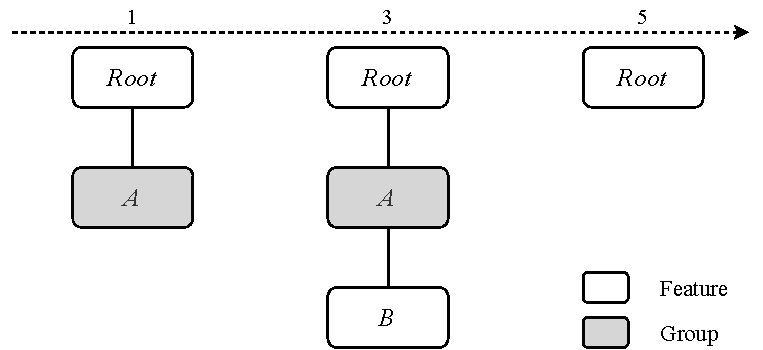
\includegraphics[width=0.7\textwidth]{AddFeatureModifiedPlan}
  \caption{Add Feature \textemdash{} modified plan}
  \label{ex:add-feature-modified-plan}
\end{figure}

If we tried to add the from 3 to 6 instead, the premise $\interval{t_n}{t_m} \inn F_e$ would fail, since the parent group only exists until 5. If a premise is false, the rule cannot be applied. 

\begin{figure}[hpbt]
    \renewcommand{\arraystretch}{1.1}
    \sossize$$\begin{array}{c}
      \ntyperule{Add-Group}
      {\\
        \interval{t_n}{t_m} \notinnr G_e \qquad \interval{t_n}{t_m} \inn F_e \qquad
        t_n < t_m\\
        \lookup{\groups{}}{\var{groupID}} = \group \\
        \lookup{\features{}}{\var{parentFeatureID}} = \feature 
      }
      {
        \textbf{addGroup}( \var{groupID}, \var{type}, \var{parentFeatureID} ) \text{ from } t_n \text{ to } t_m \shove \\
        ( \names{}, \features{}, \groups{} ) \\
        \transition \\
        \big(\names{}, \\
        \begin{aligned}
          \lookup{\features{}}{\var{parentFeatureID}} \assign \var{addChildGroup}(& \lookup{\features{}}{\var{parentFeatureID}},\, \\ 
                                                                                  & \interval{t_n}{t_m},\, \var{groupID}), 
        \end{aligned}\\ 
        \begin{aligned}
          \lookup{\groups{}}{\var{groupID}} \assign 
          \var{setGroupAttributes}(& \lookup{\groups{}}{\var{groupID}}, \var{type}, \\
                                   & \var{parentFeatureID} )\big)
         \end{aligned}
      }
    \end{array}$$
    \caption{The \rulefont{Add-Group} rule}
    \label{rule:add-group}
\end{figure}

\begin{figure}[hpbt]
  \begin{minted}[escapeinside=||]{text}
addChildGroup|$\left(\feature, \,\interval{t_{start}}{t_{end}}, \, \var{groupID}\right)$|
= |$\left(F_e,\, F_n,\, F_t,\, F_p,\, \lookup{F_c}{\interval{t_{start}}{t_{end}}} \addassign \var{groupID}\right)$|
  \end{minted}
  \caption{\var{addChildGroup}}
  \label{fun:add-child-group}
\end{figure} 

\begin{figure}[hpbt]
  \begin{minted}[escapeinside=||]{text}
setGroupAttributes|$\big(\group, \, \interval{t_{start}}{t_{end}}, \, \var{type}$|
                |$, \var{parentFeatureID}\big)$|
= |$($| |$G_e \cup \set{\interval{t_{start}}{t_{end}}}$|
  , |$\lookup{G_t}{\interval{t_{start}}{t_{end}}}$| |$\assign$| type
  , |$\lookup{G_p}{\interval{t_{start}}{t_{end}}}$| |$\assign$| parentFeatureID
  , |$G_c )$|
  \end{minted}
  \caption{\var{setGroupAttributes}}
  \label{fun:set-group-attributes}
\end{figure}

\newpage
\section{Add Group Rule}
\label{sec:add-group-rule}
In Section~\ref{sec:operations} we have defined the \textbf{addGroup} operation, which adds a group to a feature model evolution plan during a given interval. The rule in Figure~\ref{rule:add-group} describes the conditions which must be in place to add a group to the FMEP during an interval ($\interval{t_n}{t_m}$), as well as how to update the model if all the premises are true.

The group must not already exist in the plan during the interval ($\interval{t_n}{t_m} \notinnr G_e$), and the parent feature must exist for the duration of the interval ($\interval{t_n}{t_m} \inn F_e$). Lastly, the interval must fulfil the condition $t_n < t_m$, meaning that it starts before it ends. 

If all the premises hold, the model is updated according to the semantics of the \textbf{addGroup} operation. The group ID is added to the parent feature's map of child groups with the interval as key, and the attributes specified are added to the group entry in the $\groups$ map. This is achieved by using the $\var{add\-Child\-Group}$ function (in Figure~\ref{fun:add-child-group}), which is extremely similar to $\var{add\-Child\-Feature}$, and adds the group to its new parent feature, and the $\var{set\-Group\-Attributes}$ function (in Figure~\ref{fun:set-group-attributes}), which is similar to $\var{set\-Feature\-Attributes}$ and updates the group entry with the attributes given in the operation.

\section{Remove Feature Rule}
\label{sec:remove-feature-rule}

Recall that the \textbf{removeFeature} operation removes a feature at a given time, as defined in Section~\ref{sec:operations}. Figure \ref{rule:remove-feature} shows the semantics of removing a feature with ID $\var{feature\-ID}$ at time $t_n$. We find the time point when the feature was to be removed in the original plan by looking up the interval containing $t_n$ in the feature's $\map{existence}$ set $\interval{t_{e_1}}{t_{e_2}}$. The interval in which the new plan is different from the original is then $\interval{t_n}{t_{e_2}}$. We verify that the feature does not have any child groups during the affected interval ($\lookup{F_c}{\interval{t_{n}}{t_{e_2}}} = \emptyset$). We furthermore check that the feature has only a single name, type, and parent during the interval. This means that the original plan did not change the feature's name, type, or parent during this time. If these conditions all hold, we update the interval-based feature model by clamping all the relevant intervals to $t_n$, i.e. shortening them to end at $t_n$. To achieve this, we use helper functions. The $\var{clamp\-Interval}$ function (in Figure~\ref{fun:clamp-interval}) takes an interval map and a time point $t_n$, and shortens the key containing $t_n$ to end at $t_n$. Note that it assumes that the interval map contains exactly one key containing the time point. The premises in the rule ensure that this is true. We use the $\var{clamp\-Feature}$ function (in Figure~\ref{fun:clamp-feature}) to update the feature entry, ending all its interval map keys containing $t_n$ at $t_n$ by using $\var{clamp\-Interval}$ and $\var{clamp\-Set\-Interval}$ (in Figure~\ref{fun:clamp-set-interval}). The helper function $\var{clamp\-Set\-Interval}$ does the same as $\var{clamp\-Interval}$, but shortens a member of an interval set instead of a key in an interval map. To remove the feature from its parent group's child feature map, we use the helper function $\var{remove\-Feature\-At}$ (in Figure~\ref{fun:remove-feature-at}). This function applies $\var{clamp\-Interval\-Value}$ (in Figure~\ref{fun:clamp-interval-value}) to the group's child feature map. The $\var{clamp\-Interval\-Value}$ function removes the feature from the mapping containing the time point given, and adds it to the set at the key which ends at the same time point.

\begin{figure}
    \renewcommand{\arraystretch}{1.1}
    \sossize$$\begin{array}{c}
      \ntyperule{Remove-Feature}
      {\\
        \containing{F_e}{t_n} = \set{\interval{t_{e_1}}{t_{e_2}}} \qquad
        \lookup{F_c}{\interval{t_{n}}{t_{e_2}}} = \emptyset \\
        \lookup{F_n}{\interval{t_n}{t_{e_2}}} = \set{\var{name}} \qquad
        \lookup{F_t}{\interval{t_n}{t_{e_2}}} = \set{\var{type}} \qquad
        \lookup{F_p}{\interval{t_n}{t_{e_2}}} = \set{\var{parent\-Group\-ID}} \\
        \lookup{\features{}}{\var{feature\-ID}} = \feature \\
        \lookup{\groups{}}{\var{parent\-Group\-ID}} = \group
      }
      {
        \textbf{removeFeature}\left( \var{feature\-ID}\right) \text{ at } t_n \shove \\
        (\names{}, \features{}, \groups{}) \\
        \transition \\
        \big(\lookup{\names{}}{\var{name}} \assign \var{clamp\-Interval}(\lookup{\names{}}{\var{name}}, t_n),\\
        \lookup{\features{}}{\var{feature\-ID}} \assign \var{clamp\-Feature}(\lookup{\features{}}{\var{feature\-ID}}, t_n) ,\\
      \lookup{\groups{}}{\var{parent\-Group\-ID}} \assign \var{remove\-Feature\-At}\left(\lookup{\groups}{\var{parent\-Group\-ID}}, \var{feature\-ID}, t_n\right)\big)
      }
    \end{array}$$
    \caption{The \rulefont{Remove-Feature} rule}
    \label{rule:remove-feature}
\end{figure}

\begin{figure}
\begin{minipage}[t]{0.5\textwidth}
  \begin{minted}[escapeinside=||]{text}
clampInterval|$\left( \map{map}, \, t_c \right)$|
  = |$\lookup{\map{map}'}{\interval{t_{start}}{t_c}} \assign v$|
  where |$\set{\interval{t_{start}}{t_{end}}} = \containing{\map{map}}{t_c}$|
        |$\set{v} = \lookup{\map{map}}{t_c}$|
        |$\map{map}' = \map{map} \remove \interval{t_{start}}{t_{end}}$|
  \end{minted}
  \captionof{figure}{\var{clampInterval}}
  \label{fun:clamp-interval}
\end{minipage}
\begin{minipage}[t]{0.5\textwidth}
  \begin{minted}[escapeinside=||]{text}
clampIntervalValue|$\left( \map{map}, \, t_c ,\, v\right)$|
  = |$\lookup{\map{map}'}{\interval{t_{start}}{t_c}} \addassign v$|
  where |$\set{\interval{t_{start}}{t_{end}}} = \containingvalue{\map{map}}{t_c}{v}$|
        |$\map{map}' = \map{map} \removevalue{v} \interval{t_{start}}{t_{end}}$|
        |$$|
  \end{minted}
  \captionof{figure}{\var{clampIntervalValue}}
  \label{fun:clamp-interval-value}
\end{minipage}
\\

\begin{minipage}[t]{0.5\textwidth}
  \begin{minted}[escapeinside=||]{text}
     |$$|
clampSetInterval|$\left( \map{IS}, \, t_c \right)$|
  = |$\map{IS}' \cup \set{\interval{t_{start}}{t_c}}$|
  where |$\set{\interval{t_{start}}{t_{end}}} = \containing{\map{IS}}{t_c}$|
        |$\map{IS}' = \map{IS} \remove \interval{t_{start}}{t_{end}}$|
     |$$|
  \end{minted}
  \captionof{figure}{\var{clampSetInterval}}
  \label{fun:clamp-set-interval}
\end{minipage}
\begin{minipage}[t]{0.5\textwidth}
  \begin{minted}[escapeinside=||]{text}
     |$$|
clampFeature|$\left(\feature, \, t_c \right)$|
  = |$(\var{clampSetInterval}(F_e, t_c)  $|
    |$, \var{clampInterval}(F_n, t_c)$|
    |$, \var{clampInterval}(F_t, t_c)$|
    |$, \var{clampInterval}(F_p, t_c)$|
    |$, F_c)$|
  \end{minted}
  \captionof{figure}{\var{clampFeature}}
  \label{fun:clamp-feature}
\end{minipage}

\begin{minipage}{0.5\textwidth}
  \begin{minted}[escapeinside=||]{text}
     |$$|
clampGroup|$\left(\group, \, t_c \right)$|
  = |$(\var{clampSetInterval}(G_e)  $|
    |$, \var{clampInterval}(G_t, t_c)$|
    |$, \var{clampInterval}(G_p, t_c)$|
    |$, G_c)$|
  \end{minted}
  \captionof{figure}{\var{clampGroup}}
  \label{fun:clamp-group}
\end{minipage}

\begin{minipage}{0.6\textwidth}
  \begin{minted}[escapeinside=||]{text}
    |$$|
    |$$|
removeFeatureAt|$\big(\group, \var{featureID}, t_c \big)$|
  = |$\big(G_e, G_t, G_p$|
    |$,\var{clampIntervalValue}\left(G_c, t_c, \var{featureID}\right)\big)$|
  \end{minted}
  \captionof{figure}{\var{removeFeatureAt}}
  \label{fun:remove-feature-at}
\end{minipage}

\begin{minipage}{0.6\textwidth}
  \begin{minted}[escapeinside=||]{text}
    |$$|
    |$$|
removeGroupAt|$\left(\feature, \var{groupID}, t_c \right)$|
  = |$\big(F_e, F_n, F_t, F_p$|
    |$,\var{clampIntervalValue}\left(F_c, t_c, \var{groupID}\right)\big)$|
  \end{minted}
  \captionof{figure}{\var{removeGroupAt}}
  \label{fun:remove-group-at}
\end{minipage}
\end{figure}

\begin{figure}[htbp]
    \renewcommand{\arraystretch}{1.1}
    \sossize$$\begin{array}{c}
      \ntyperule{Remove-Group}
      {\\
        \containing{G_e}{t_n} = \set{\interval{t_{e_1}}{t_{e_2}}} \qquad
        \lookup{G_c}{\interval{t_{n}}{t_{e_2}}} = \emptyset \\
        \lookup{G_t}{\interval{t_n}{t_{e_2}}} = \set{\var{type}} \qquad
        \lookup{G_p}{\interval{t_n}{t_{e_2}}} = \set{\var{parentFeatureID}} \\
        \lookup{\groups{}}{\var{groupID}} = \group \\
        \lookup{\features{}}{\var{parentFeatureID}} = \feature
      }
      {
        \textbf{removeGroup}\left( \var{groupID}\right) \text{ at } t_n \shove \\
        (\names{}, \features{}, \groups{}) \\
        \transition \\
        \big(\names{} ,\\
          \lookup{\features{}}{\var{parentFeatureID}} \assign \var{removeGroupAt}\left(\lookup{\features}{\var{parentFeatureID}}, \var{groupID}, t_n\right) ,\\
        \lookup{\groups{}}{\var{groupID}} \assign \var{clampGroup}\left(\lookup{\groups{}}{\var{groupID}}, t_n\right) \big)
      }
    \end{array}$$
    \caption{The \rulefont{Remove-Group} rule}
  \label{rule:remove-group}
\end{figure}


\section{Remove Group Rule}
\label{sec:remove-group-rule}
We defined the operation \textbf{removeGroup} in Section~\ref{sec:operations}. The operation removes a group at a given time point, similarly to \textbf{removeFeature}.

The $\rulefont{Remove-Group}$ rule in Figure~\vref{rule:remove-group} describes the semantics of removing a group in an interval-based feature model. The temporal scope is identified as the existence interval containing the time point for removal. In that interval, the group should not have any children, and there cannot be plans to change the type or move the group within the interval. We check the latter by looking up the type and parent feature during the interval; if the set contains only one type/parent feature then the type and parent feature do not change. 

We use the helper functions $\var{remove\-Group\-At}$ (in Figure~\ref{fun:remove-group-at}) and $\var{clamp\-Group}$ (in Figure~\ref{fun:clamp-group}) to update the interval-based feature model.  The $\var{remove\-Group\-At}$ function, similar to $\var{remove\-Feature\-At}$, takes the parent feature entry, the group ID, and a time point $t_c$, and applies \var{clampIntervalValue} to the parent feature's child group map. The $\var{clamp\-Group}$ function does the same as $\var{clamp\-Feature}$, but to a group entry. After applying these to the interval-based feature model, the group is removed from the model during the temporal scope.

\begin{figure}[htbp]
    \renewcommand{\arraystretch}{1.1}
    \sossize$$\begin{array}{c}
      \ntyperule{Move-Feature}
      {\\
        \neg \var{createsCycle} \qquad
        \containing{F_p}{t_n} = \set{\interval{t_{p_1}}{t_{p_2}}} \\
        \lookup{F_p}{\interval{t_n}{t_{p_2}}} = \set{\var{oldParentID}} \qquad
        \interval{t_n}{t_{p_2}} \inn G_e\\
        \\
        \begin{aligned}
          \forall \interval{t_{f_1}}{t_{f_2}} & \in \overlapping{F_t}{t_n}{t_{p_2}}
          \forall \interval{t_{g_1}}{t_{g_2}} \in \lookup{G_t}{\clamp{\interval{t_{f_1}}{t_{f_2}}}{t_n}{t_{p_2}}}_{\overlap{}} \\
          \forall \var{ft} & \in \lookup{F_t}{\interval{t_{f_1}}{t_{f_2}}}
          \forall \var{gt} \in \lookup{G_t}{\interval{t_{g_1}}{t_{g_2}}}
          \left(\var{compatibleTypes}(\var{gt},\, \var{ft}) \right)
        \end{aligned} \\
      \\
      \lookup{\features{}}{\var{featureID}} = \feature \\
        \lookup{\groups{}}{\var{newParentID}} = \group
      }
      {
        \textbf{moveFeature}\left( \var{featureID, newParentID}\right) \text{ at } t_n \shove \\
        (\names{}, \features{}, \groups{}) \\
        \transition \\
        \big(\names,\\
          \lookup{\features{}}{\var{featureID}} \assign \left( F_e,\, F_n,\, F_t,\, 
        \lookup{\var{clampInterval}(F_p, t_n)}{\interval{t_n}{t_{p_2}}} \assign \var{newParentID},\, F_c \right), \\

        \lookup{\big(\lookup{\groups{}}{\var{oldParentID}} \\
        \assign \var{removeFeatureAt}\left(\lookup{\groups{}}{\var{oldParentID}}, \var{featureID}, t_n\right)\big)}{\var{newParentID}} \\
        \assign 
      \var{addChildFeature}(\lookup{\groups{}}{\var{newParentID}}, \interval{t_n}{t_{p_2}}, \var{featureID})
        }
    \end{array}$$
    \caption{The \rulefont{Move-Feature} rule}
  \label{rule:move-feature}
\end{figure}

\section{Move Feature Rule}
\label{sec:move-feature-rule}

In Section~\ref{sec:operations}, we defined the \textbf{moveFeature} operation to move a feature from a group to a new group at a given time. See Figure~\vref{rule:move-feature} for the semantics of the \textbf{moveFeature} operation. The premise $\neg \var{createsCycle}$ refers to the cycle detection algorithm described in Section~\vref{sub:move-algorithm}. A concrete implementation of the algorithm can be found on GitHub\footnote{\url{https://github.com/idamotz/Master/blob/master/soundness-checker/}}. 

The premise $\containing{F_p}{t_n} = \set{\interval{t_{p_1}}{t_{p_2}}}$ locates the scope of the operation, namely $\interval{t_n}{t_{p_2}}$. The ID of the feature's former parent group is identified in the premise $\lookup{F_p}{\interval{t_n}{t_{p_2}}} = \set{\var{oldParentID}}$ for the purpose of updating the $\groups{}$ map. The premise $\interval{t_n}{t_{p_2}} \inn G_e$ ensures that the new parent exists during the entire temporal scope.

As the plan may contain several type changes for both the feature being moved and its new parent, we must check that the types they have at the same time are compatible. This is achieved by the following premise
\begin{align*}
  \forall \interval{t_{f_1}}{t_{f_2}} & \in \overlapping{F_t}{t_n}{t_{p_2}}
  \forall \interval{t_{g_1}}{t_{g_2}} \in \lookup{G_t}{\clamp{\interval{t_{f_1}}{t_{f_2}}}{t_n}{t_{p_2}}}_{\overlap{}} \\
  \forall \var{ft} & \in \lookup{F_t}{\interval{t_{f_1}}{t_{f_2}}}
  \forall \var{gt} \in \lookup{G_t}{\interval{t_{g_1}}{t_{g_2}}}
  \left(\var{compatibleTypes}(\var{gt},\, \var{ft}) \right)
\end{align*}
It says that for each interval key overlapping the temporal scope in the feature's type map, then for each interval in the group's type map overlapping the aforementioned key and restricted by the temporal scope, then for all types mapped to by those keys, those types must be compatible. This ensures that we are not too strict, because we check only those combinations of types which the feature and its new parent group have at the same time, further restricted by the temporal scope.

If all the premises hold, then the interval-based feature model is updated to reflect it. The feature's parent group map is updated by shortening the interval mapped to the former parent's ID to end at $t_n$, and adding a new mapping $\intervalmapping{t_n}{t_{p_2}}{\var{newParentID}}$.

The feature is removed from the previous parent's ($\var{oldParentID}$) set of child features during the temporal scope, and the feature is added to the new parent's set of child features during the same interval. 

\begin{figure}[htpb]
  \centering
  \textbf{Original plan}
  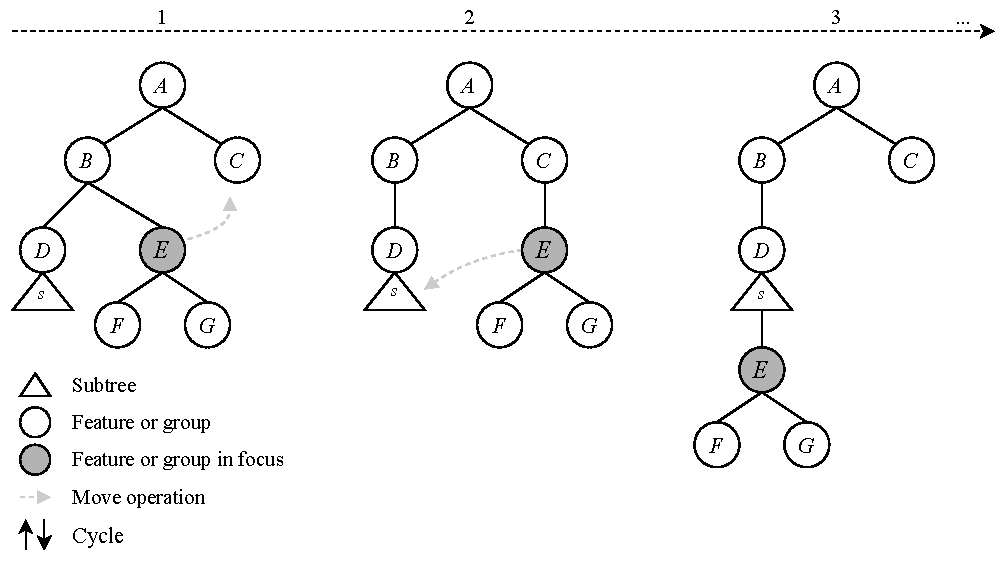
\includegraphics[width=0.9\textwidth]{MoveParadox1}
  \bigskip

  apply \textbf{moveFeature}($D$, $F$) at 1
  \bigskip 
  
  \textbf{Modified plan}
  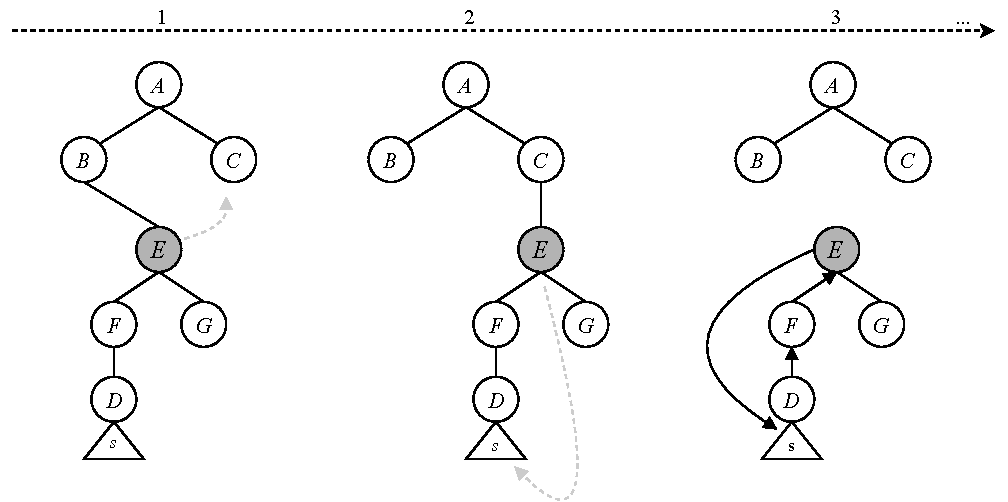
\includegraphics[width=0.9\textwidth]{MoveParadox2}
  \caption{Illustration of move paradox}
  \label{ex:illustration-move-algo}
\end{figure}


\subsection{Algorithm for Detecting Cycles Resulting from \textbf{Move} Operations}
\label{sub:move-algorithm}

Compared with the other operations, \textbf{moveFeature} and \textbf{moveGroup} require extensive verification, as moving a feature or a group may cause cycles at the time of the move or at some later point. Since cycles violate only the tree structure of the feature model evolution plan, we abstract away from groups and features, viewing both as nodes.  

In Figure~\vref{ex:illustration-move-algo}, we show an example of a cycle arising from a move operation. In the original plan, the marked node $E$ is moved to $C$ at time 2, and to \emph{some node} in node $D$'s subtree $s$. In the modified plan, $D$ (and its subtree $s$) has been moved to node $F$. There is no cycle at time $1$ or $2$, but at time 3, when $E$ is moved to $s$, it causes a cycle. At time $1$, the new ancestors of $D$ are $F$, $G$, and $E$. At time $2$, the new ancestors are still $F$, $G$, and $E$, but $C$ is added to the list, since $C$ was not an ancestor of $D$ in the original plan. When $E$ is then moved to $D$'s subtree $s$, it causes a cycle, since $E$ now has $F$ as an ancestor.

Following is a description of an algorithm intended to ensure that adding a \textbf{moveFeature} or \textbf{moveGroup} operation does not cause a cycle.

Let $n$ be the node to be moved and $c_1$ the target node, i.e. $n$'s new parent node. Furthermore, let $t_1$ be the time point at which this operation is inserted, and $t_e$ the time point where $n$ is moved next or removed, or $\forever$. We use the function $\var{ancestors}(IBFM, \var{node}, \var{time})$ (see Figure~\vref{fun:ancestors}), written in Haskell-like syntax, which takes the interval-based feature model, a node, and a time point and returns a list of $\var{node}$'s ancestors at time point $\var{time}$.

First, check whether $n \in \texttt{ancestors}(IBFM, c_1, t_1)$. If this is the case, report that the move causes a cycle and terminate. 

Next, find a list of critical nodes. 
Let $A_n = \texttt{ancestors}(IBFM, n, t_1) = [a_1, a_2, \dots, SN, \dots, r]$ and $A_{c_1} = \texttt{ancestors}(IBFM, c_1, t_1) = [c_2, c_3, \dots, c_n, SN, \dots, r]$ with $SN$ the first common ancestor of $n$ and $c_1$. The list of critical nodes is then $C = [c_1, c_2, \dots, c_n]$, which is essentially the list of $n$'s new ancestors after the move. 

\textbf{Repeat this step until the algorithm terminates:}

Look for the first move of one of the critical nodes. If no such moves occur until $t_e$, the operation causes no paradoxes, and the algorithm terminates successfully.  
  Suppose there is a `move` operation scheduled for $t_k$, with $t_1 < t_k < t_e$, where $c_i$ is moved to $k$. There are two possibilities:  
  \begin{enumerate}
    \item $k$ is in $n$'s subtree, which is equivalent to $n \in \texttt{ancestors}(IBFM, k, t_k)$. Report that the move will cause a cycle and terminate. 
\item $k$ is not in $n$'s subtree, so this move is safe. Let $A_k = \texttt{ancestors}(IBFM, k, t_k) = [k_1, k_2, \dots, k_n, SN', \dots, r]$, with SN' the first common element of $A_k$ and $A_n$. Update the list of critical nodes to $[c_1, \dots, c_i, k_1, \dots, k_n]$.
  \end{enumerate}

\begin{figure}[h]
  \begin{minted}[escapeinside=||]{text}
ancestors|$\left((\names{}, \features{}, \groups{}), \, \var{featureID}, t_n \right)$| 
  = case parentGroup of
        { parentGroupID } |$ \rightarrow $| 
             parentGroupID : ancestors|$((\names, \features{}, \groups{}),$|
                                        |$\var{parentGroupID}, t_n)$|
        |$ \emptyset \rightarrow $| []
  where |$\feature = \lookup{\features{}}{\var{featureID}}$|
        parentGroup |$ = \lookup{F_p}{t_n} $|

ancestors|$\left((\names{}, \features{}, \groups{}), \, \var{groupID}, t_n \right)$| 
  = parentFeatureID : ancestors|$((\names{}, \features{}, \groups{}),$|
                                 |$\var{parentFeatureID}, t_n )$| 
  where |$\group \assign     \lookup{\groups{}}{\var{groupID}}$|
        { parentFeatureID } |$ \assign \lookup{G_p}{t_n} $|
  \end{minted}
  \caption{\var{ancestors}}
  \label{fun:ancestors}
\end{figure}

\begin{figure}[htbp]
    \renewcommand{\arraystretch}{1.1}
    \sossize$$\begin{array}{c}
      \ntyperule{Move-Group}
      {\\
        \neg \var{createsCycle} \qquad
        \containing{G_p}{t_n} = \set{\interval{t_{p_1}}{t_{p_2}}} \\
        \interval{t_n}{t_{p_2}} \inn F_e \qquad
        \lookup{G_p}{\interval{t_n}{t_{p_2}}} = \set{\var{oldParentID}} \\
        \lookup{\groups{}}{\var{groupID}} = \group \\
        \lookup{\features{}}{\var{newParentID}} = \feature 
      }
      {
        \textbf{moveGroup}\left( \var{groupID, newParentID}\right) \text{ at } t_n \shove \\
        (\names{}, \features{}, \groups{}) \\
        \transition \\
        \big(\names,\\
        \lookup{\big(\lookup{\features{}}{\var{oldParentID}} \\
        \assign \var{removeGroupAt}(\lookup{\features{}}{\var{oldParentID}}, \interval{t_n}{t_{p_2}}, \var{groupID})\big)}{\var{newParentID}} \\
        \assign 
      \var{addChildGroup}\left(\lookup{\features{}}{\var{newParentID}}, \var{groupID}, t_n\right), \\
        \lookup{\groups{}}{\var{groupID}} \assign \left( G_e,\, G_n,\, G_t,\, 
        \lookup{\var{clampInterval}(G_p, t_n)}{\interval{t_n}{t_{p_2}}} \assign \var{newParentID},\, G_c \right)}
    \end{array}$$
    \caption{The \rulefont{Move-Group} rule}
  \label{rule:move-group}
\end{figure}


\section{Move Group Rule}
\label{sec:move-group-rule}
The \textbf{moveGroup} operation moves a group from its parent feature to a new parent, as explained in Section~\ref{sec:operations}.

See Figure~\vref{rule:move-group} for the semantics of the \textbf{moveGroup} operation. The rule is similar to the \rulefont{Move-Feature} rule, but it differs in that it does not have a check for types. This is because there can only be a conflict between a parent group and a child feature, not a parent feature and a child group. Since only the latter relation changes in this rule, it is not necessary to check that the types are compatible. The model is updated similarly to the way it is done in the \rulefont{Move-Feature} rule. 

\begin{figure}[htbp]
    \renewcommand{\arraystretch}{1.1}
    \sossize$$\begin{array}{c}
      \ntyperule{Change-Feature-Variation-Type}
      {\\
        \var{featureID} \neq RootID \qquad
        \containing{F_t}{t_n} = \set{\interval{t_{t_1}}{t_{t_2}}} % Temporal scope = [t_n, t_t_2)
        \\
        \\
        \begin{aligned}
          \forall \interval{t_{p_1}}{t_{p_2}} & \in \overlapping{F_p}{t_n}{t_{t_2}}  \\ % for all parent intervals overlapping the temporal scope
          \forall p & \in \lookup{F_p}{\interval{t_{p_1}}{t_{p_2}}}  \\% for all parent groups (always exactly one) in the parent interval
          \forall t & \in \, \var{getTypes}\left(\lookup{\groups}{p}, \clamp{\interval{t_{p_1}}{t_{p_2}}}{t_n}{t_{t_2}}\right)  \\
                    & \big(\var{compatibleTypes}(t, \var{type})\big) 
        \end{aligned}\\
        \\
        \lookup{\features{}}{\var{featureID}} = \feature
      }
      {
        \textbf{changeFeatureVariationType}\left( \var{featureID}, \var{type}\right) \text{ at } t_n \shove \\
        (\names{}, \features{}, \groups{}) \\
        \transition \\
        (\names{}, \\
        \lookup{\features{}}{\var{featureID}} \assign \left( F_e,\, F_n,\, 
        \lookup{\var{clampInterval}(F_t, t_n)}{\interval{t_n}{t_{t_2}}} \assign \var{type},\, F_p,\, F_c \right),
        \\ \groups{})
      }
    \end{array}$$
    \caption{The \rulefont{Change-Feature-Variation-Type} rule}
    \label{rule:change-feature-varation-type}
\end{figure}

\begin{figure}[htbp]
  \begin{minted}[escapeinside=||]{text}
getTypes|$\left(\group, \, \interval{t_n}{t_m} \right) = \lookup{G_t}{\interval{t_n}{t_m}}$|
getTypes|$\left(\feature, \, \interval{t_n}{t_m} \right) = \lookup{G_t}{\interval{t_n}{t_m}}$|
  \end{minted}
  \caption{\var{getTypes}}
  \label{fun:get-types}
\end{figure}

\section{Change Feature Variation Type Rule}
\label{sec:change-feature-variation-type-rule}
The operation \textbf{changeFeatureVariationType} is defined in Section~\ref{sec:operations} to update a feature's type at some time point in the evolution plan.

The rule in Figure~\vref{rule:change-feature-varation-type} shows the semantics of changing the feature variation type of the feature with ID $\var{feature\-ID}$ at time $t_n$. The first premise $\var{feature\-ID} \neq Root\-ID$ ensures that we are not attempting to modify the type of the root feature, which should always be \mandatory{}. The second premise ($\containing{F_t}{t_n} = \set{\interval{t_{t_1}}{t_{t_2}}}$) identifies the upper bound of the temporal scope, $t_{t_2}$. This is when the feature type was originally planned to change. If there is no such planned change, then $t_{t_2} = \forever$. The temporal scope is then $\interval{t_n}{t_{t_2}}$ as defined in the \nameref{sec:scope} section (Section~\ref{sec:scope}). %TODO: maybe re-add vref
The next premise is a little convoluted, but its intent is easier to understand:
\begin{align*}
   \forall \interval{t_{p_1}}{t_{p_2}} & \in \overlapping{F_p}{t_n}{t_{t_2}}  \\ % for all parent intervals overlapping the temporal scope
   \forall p & \in \lookup{F_p}{\interval{t_{p_1}}{t_{p_2}}}  \\% for all parent groups (always exactly one) in the parent interval
   \forall t & \in \, \var{getTypes}\left(\lookup{\groups}{p}, \clamp{\interval{t_{p_1}}{t_{p_2}}}{t_n}{t_{t_2}}\right)  \\
            & \big(\var{compatibleTypes}(t, \var{type})\big) 
\end{align*}
It checks that all the types a parent group has \emph{while it is the parent of the feature}, restricted by the temporal scope, has a type which is compatible with the new type of the feature. This is necessary as the feature may potentially move around several times during the temporal scope, and the various parent groups could change their types often. It uses the helper function $\var{get\-Types}$ (in Figure~\ref{fun:get-types}), which takes a group or feature entry and an interval, and returns the types the feature or group has during the interval.

If all the premises are true, then the $\features{}$ map is updated at $\var{featureID}$ by shortening the interval key for the original type at $t_n$ using $\var{clamp\-Interval}$, and assigning the new type to the temporal scope $\interval{t_n}{t_{t_2}}$. 

\begin{figure}
    \renewcommand{\arraystretch}{1.1}
    \sossize$$\begin{array}{c}
      \ntyperule{Change-Group-Variation-Type}
      {\\
        \containing{G_t}{t_n} = \set{\interval{t_{t_1}}{t_{t_2}}} % Temporal scope = [t_n, t_t_2)
        \\
        \\
        \begin{aligned}
          \forall \interval{t_{c_1}}{t_{c_2}} & \in \overlapping{G_c}{t_n}{t_{t_2}}\\ % for all parent intervals overlapping the temporal scope 
          \forall c & \in \, \bigcup \lookup{G_c}{\interval{t_{c_1}}{t_{c_2}}}\\ % for all child features in the child interval
          \forall t & \in \, \var{getTypes}\left(\lookup{\features}{c}, \clamp{\interval{t_{c_1}}{t_{c_2}}}{t_n}{t_{t_2}}\right) \\ % for all the types of the child features during the temporal scope
                    & \big(\var{compatibleTypes}(\var{type}, t)\big)
      \end{aligned}\\
         \\

        \lookup{\groups{}}{\var{groupID}} = \group
      }
      {
        \textbf{changeGroupVariationType}\left( \var{groupID}, \var{type}\right) \text{ at } t_n \shove \\
        (\names{}, \features{}, \groups{}) \\
        \transition \\
        (\names{}, \features{}, \\
        \lookup{\groups{}}{\var{groupID}} \assign \left( G_e,\, \lookup{\var{clampInterval}(G_t, t_n)}{\interval{t_n}{t_{t_2}}} \assign \var{type},\, G_p,\, G_c \right))
      }
    \end{array}$$
    \caption{The \rulefont{Change-Group-Variation-Type} rule}
  \label{rule:change-group-varation-type}
\end{figure}

\section{Change Group Variation Type Rule}
\label{sec:change-group-variation-type-rule}
The operation \textbf{changeGroupVariationType} changes the type of a group at a given time point, as defined in Section~\ref{sec:operations}. The rule in Figure~\vref{rule:change-group-varation-type} is similar to the \textbf{changeFeatureVariationType} rule in Figure~\vref{rule:change-feature-varation-type}, and shows the semantics of changing the type of a group. In a similar way to the aforementioned \rulefont{Change-Feature-Variation-Type} rule, it verifies that the types of all the child groups during the affected interval are compatible with the new group type. If they are compatible, the group entry is updated with the new type during the temporal scope.

\begin{figure}[htbp]
    \renewcommand{\arraystretch}{1.1}
    \sossize$$\begin{array}{c}
      \ntyperule{Change-Feature-Name}
      {\\
        \lookup{F_n}{t_n} = \set{\var{oldName}} \qquad
        \containing{F_n}{t_n} = \set{\interval{t_{n_1}}{t_{n_2}}} \\
        \lookup{\lookup{\names{}}{\var{name}}}{\interval{t_n}{t_{n_2}}} = \emptyset \\
        \lookup{\features{}}{\var{featureID}} = \feature
      }
      {
        \textbf{changeFeatureName}\left( \var{featureID}, \var{name}\right) \text{ at } t_n \shove \\
        (\names{}, \features{}, \groups{}) \\
        \transition \\
        \Big(\lookup{\lookup{\big(\lookup{\names{}}{\var{oldName}} \assign \var{clampInterval}\left(\lookup{\names}{\var{oldName}}, t_n\right) \big)}{\var{name}}}{\interval{t_n}{t_{n_2}}} \assign \var{featureID}, \\
        \lookup{\features{}}{\var{featureID}} \assign \left( F_e,\, \lookup{\var{clampInterval}(F_n, t_n)}{\interval{t_n}{t_{n_2}}} \assign \var{name},\, F_t,\, F_p,\, F_c \right), \\
        \groups{}\Big)
      }
    \end{array}$$
    \caption{The \rulefont{Change-Feature-Name} rule}
  \label{rule:change-feature-name}
\end{figure}

\section{Change Feature Name}
\label{sec:change-feature-name}

As defined in Section~\ref{sec:operations}, the \textbf{changeFeatureName} operation changes the name of a feature at a given time point. The semantics of changing the name of a feature are shown in the \rulefont{Change-Feature-Name} rule in Figure~\vref{rule:change-feature-name}. The old name and the next planned name change are identified on the first line ($\lookup{F_n}{t_n} = \set{\var{oldName}}$ and $\containing{F_n}{t_n} = \set{\interval{t_{n_1}}{t_{n_2}}}$ respectively). Since the name must not be in use during the temporal scope, we verify that looking up the new name in the $\names{}$ map returns an empty set. The $\names{}$ map is updated by shortening the interval for the old name to end at $t_n$, and assigning the feature ID to the new name during the temporal scope. Furthermore, the $\features{}$ map is updated at the feature ID, shortening the interval for the old name and assigning the new name to the temporal scope. 


